\clearpage
\section{Numerical exploration: the supercritical pitchfork}
\begin{colbox}
	Very long description
\end{colbox}
\emph{I assumed the entire question was meant to be done numerically so everything was done in python, including the analytical part, which was done using sympy.}
\subsection{Predict Time Scale}
\begin{table}[!htb]
	\centering
	\begin{tabular}{cccccc}
		Fixed Point & Linearized & Relaxation Time & Step Size & Integration Time \\
		\hline\\
		0 & r & \(\frac{1}{\abs{r}}\) & \(\frac{1}{10\cdot\abs{r}}\) & \(\frac{10}{\abs{r}}\) \\
		\(\sqrt{r-1}\) & \(3-2r\) & \(\frac{1}{\abs{3-2r}}\) & \(\frac{1}{10\cdot\abs{3-2r}}\) & \(\frac{10}{\abs{3-2r}}\) \\
		\(-\sqrt{r-1}\) & \(3-2r\) & \(\frac{1}{\abs{3-2r}}\) & \(\frac{1}{10\cdot\abs{3-2r}}\) & \(\frac{10}{\abs{3-2r}}\)
	\end{tabular}
	\caption{Table of the fixed points and their respective linearized forms, relaxation time, step size defined as one order of magnitude less than the relaxation time, and integration time which is defined as one order of magnitude more than the relaxation time.}
\end{table}
\subsection{Run}
\begin{figure}[!htb]
	\centering
	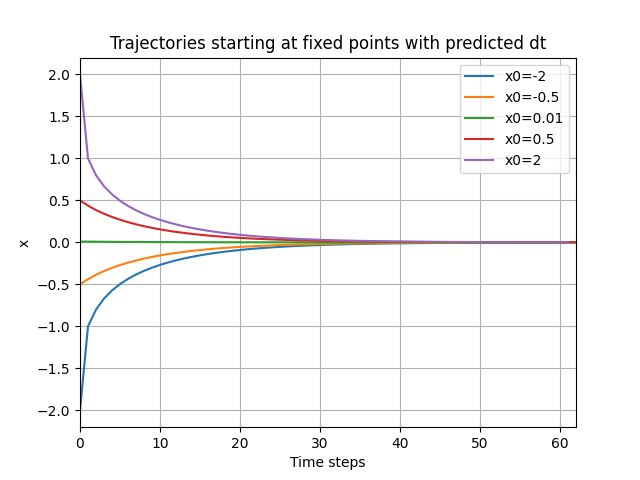
\includegraphics[width=0.75\textwidth]{q4br-1.png}
	\caption{The trajectories for the initial conditions integrated with the above parameters for \(r=-1\), meaning the relaxation time is \(1\), step size is \(1/10\), and integration time is \(10\).}
\end{figure}
\begin{figure}[!htb]
	\centering
	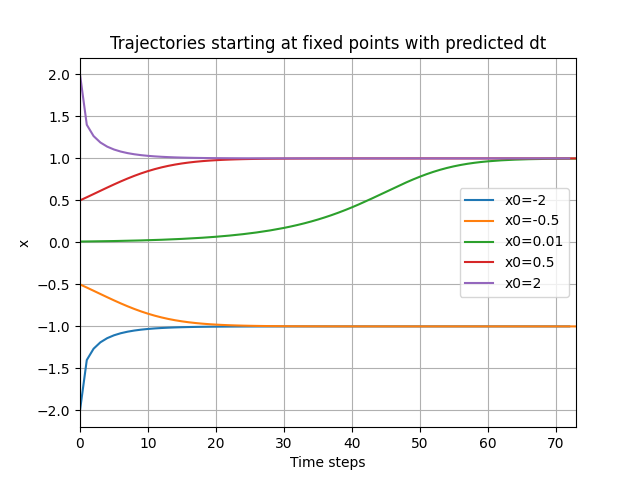
\includegraphics[width=0.75\textwidth]{q4br1.png}
	\caption{The trajectories for the initial conditions integrated with the above parameters for \(r=1\), meaning the relaxation time is \(1\), step size is \(1/10\), and integration time is \(10\).}
\end{figure}
\clearpage
\subsection{Failure Mode}
\begin{figure}[!htb]
	\centering
	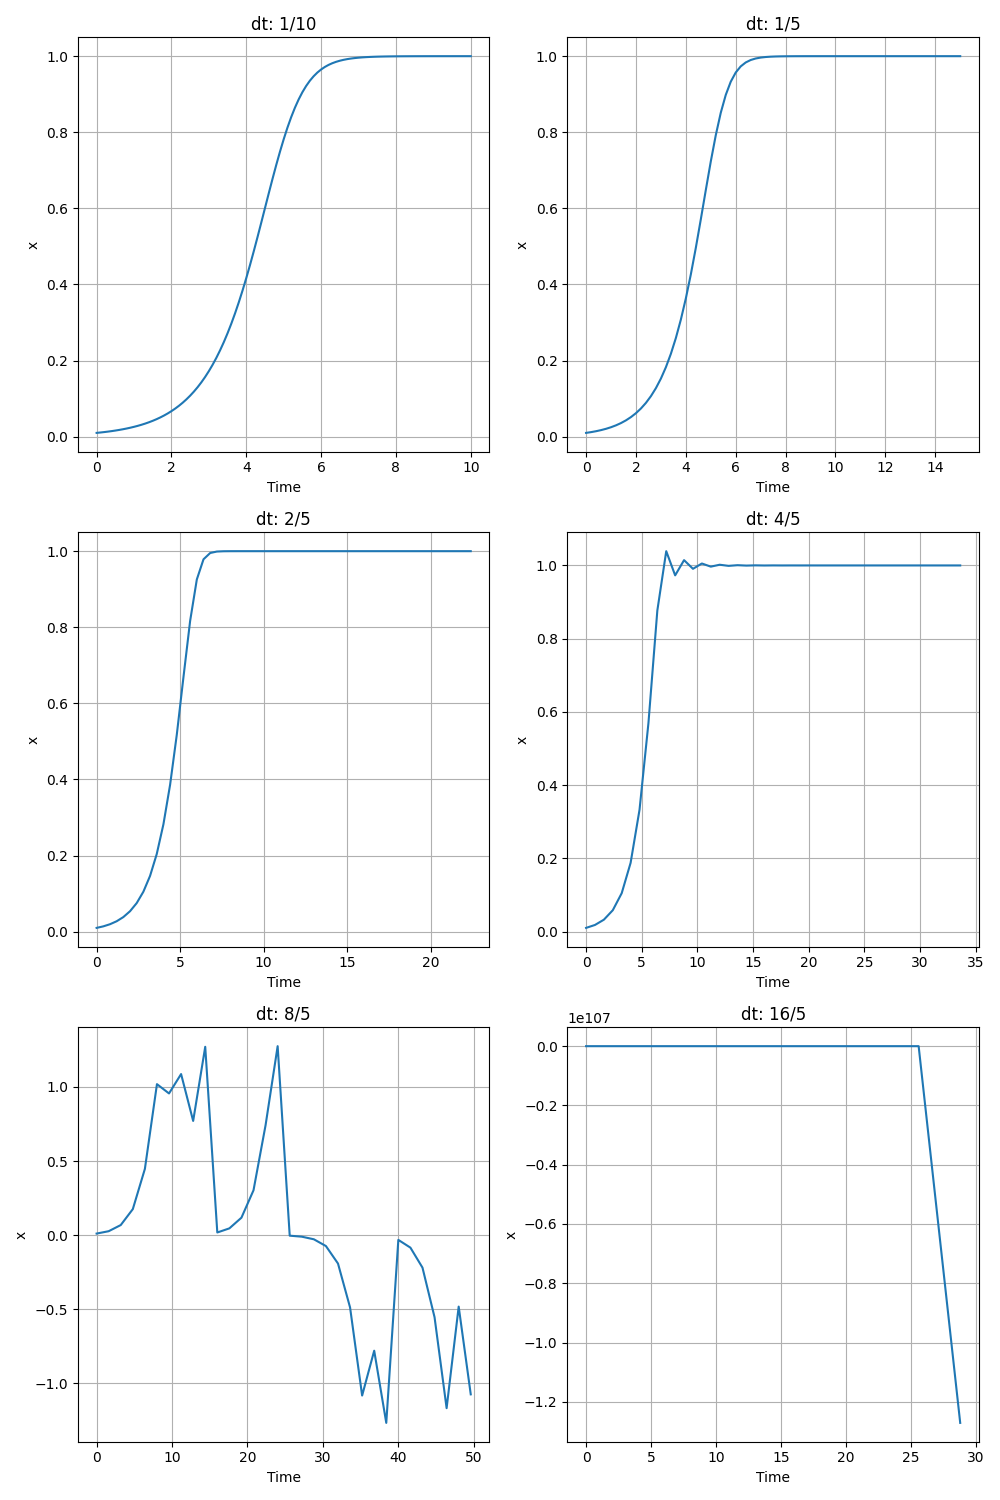
\includegraphics[width=0.85\textwidth]{failuremode.png}
	\caption{The trajectories for the fixed initial conditions with integration steps increasing by x2.}
\end{figure}
It appears that the integration breaks once it crosses \(dt=1\). This is exactly the relaxation time we found, so the rule appears to be that the time step must be smaller than the relaxation time.
\subsection{Bifurcation Diagram}
\subsubsection{Coarse r scan}
\begin{figure}[!htb]
	\centering
	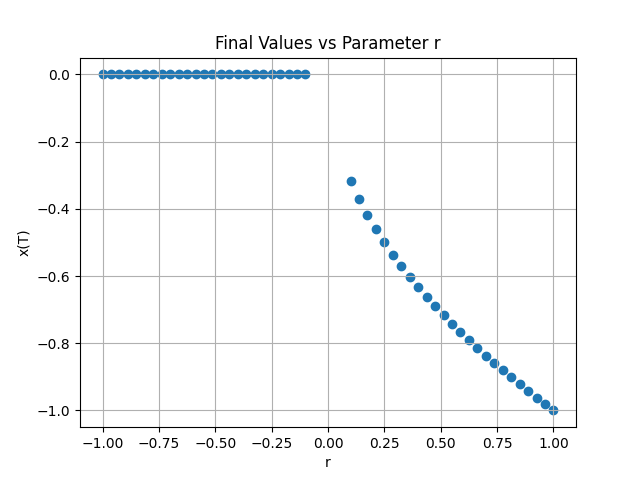
\includegraphics[width=0.75\textwidth]{coarser.png}
	\caption{Final position of x after an integration for a set of initial conditions of r selected from the range requested in the question.}
\end{figure}
This is very similar to what we saw and expect from class.
\newpage
\subsubsection{Probing \(r=0\)}
\begin{figure}[!htb]
	\centering
	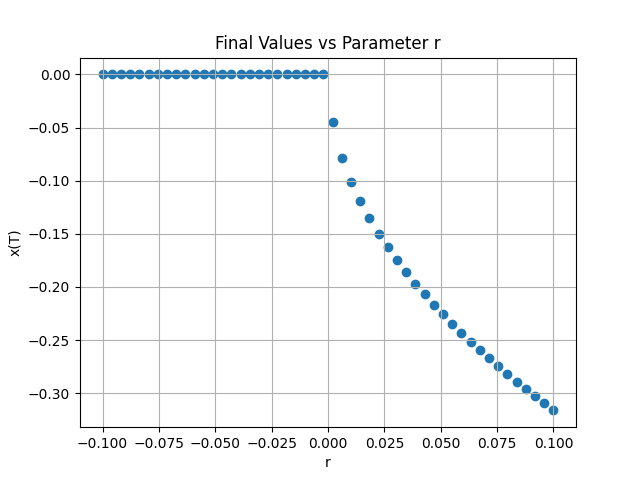
\includegraphics[width=0.75\textwidth]{finer.png}
	\caption{Final position of x after an integration for a set of initial conditions of r selected from the range requested in the question.}
\end{figure}
This is also very similar to what we saw and expect from class. I did not have issues with getting the bifurcation diagram, I'm not quite sure what I should have seen.